\documentclass[tikz,border=4pt]{standalone}
\usepackage{tikz}
\usetikzlibrary{positioning, calc, arrows.meta, fit, shapes.geometric}

\definecolor{mutblue}{RGB}{30,90,210}

\begin{document}
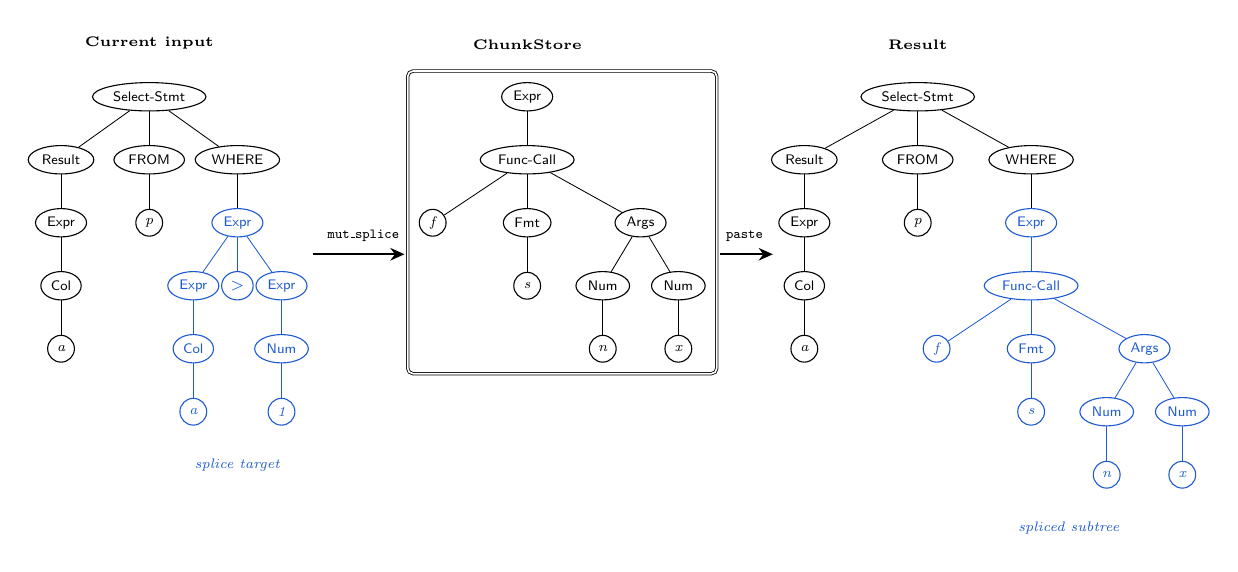
\begin{tikzpicture}[
    x=8mm, y=8mm,
    every node/.style={font=\tiny},
    nt/.style={ellipse, draw=black, line width=0.4pt,
        inner xsep=1.5pt, inner ysep=1pt, font=\tiny\sffamily,
        minimum height=3.6mm},
    op/.style={ellipse, draw=black, line width=0.4pt,
        inner xsep=0.5pt, inner ysep=1pt, font=\tiny\sffamily,
        minimum width=4mm, minimum height=3.6mm},
    lf/.style={circle, draw=black, line width=0.4pt,
        inner sep=0pt, minimum size=3.4mm, font=\tiny\itshape},
    nth/.style={ellipse, draw=mutblue, line width=0.4pt,
        inner xsep=1.5pt, inner ysep=1pt, font=\tiny\sffamily,
        minimum height=3.6mm, text=mutblue},
    oph/.style={ellipse, draw=mutblue, line width=0.4pt,
        inner xsep=0.5pt, inner ysep=1pt, font=\tiny\sffamily,
        minimum width=4mm, minimum height=3.6mm, text=mutblue},
    lfh/.style={circle, draw=mutblue, line width=0.4pt,
        inner sep=0pt, minimum size=3.4mm, font=\tiny\itshape, text=mutblue},
    te/.style={draw=black, line width=0.3pt},
    teh/.style={draw=mutblue, line width=0.3pt},
    chunkstore/.style={rectangle, draw=black, double, double distance=0.6pt,
        line width=0.3pt, rounded corners=2pt, inner sep=4pt},
    mutarrow/.style={-{Stealth[length=1.8mm,width=1.6mm]}, line width=0.6pt},
]

% ============================================================
% SECTION 1: Current input
% Tree: SELECT a FROM p WHERE a > 1   (splice target = Expr under WHERE)
% ============================================================
\begin{scope}
    \node[font=\tiny\bfseries, anchor=south] at (0,0.6) {Current input};

    \node[nt] (L-root)   at (0,0)    {Select-Stmt};
    \node[nt] (L-result) at (-1.4,-1) {Result};
    \node[nt] (L-from)   at (0,-1)    {FROM};
    \node[nt] (L-where)  at (1.4,-1)  {WHERE};

    \node[nt]  (L-expr1) at (-1.4,-2) {Expr};
    \node[lf]  (L-p)     at (0,-2)    {p};
    \node[nth] (L-expr2) at (1.4,-2)  {Expr};

    \node[nt] (L-col1) at (-1.4,-3) {Col};

    \node[nth] (L-expr3) at (0.7,-3) {Expr};
    \node[oph] (L-gt)    at (1.4,-3) {$>$};
    \node[nth] (L-expr4) at (2.1,-3) {Expr};

    \node[lf]  (L-a1)   at (-1.4,-4) {a};
    \node[nth] (L-col2) at (0.7,-4)  {Col};
    \node[nth] (L-num)  at (2.1,-4)  {Num};

    \node[lfh] (L-a2) at (0.7,-5) {a};
    \node[lfh] (L-1)  at (2.1,-5) {1};

    \foreach \a/\b in {L-root/L-result, L-root/L-from, L-root/L-where,
        L-result/L-expr1, L-from/L-p, L-where/L-expr2,
        L-expr1/L-col1, L-col1/L-a1}
        \draw[te] (\a) -- (\b);
    \foreach \a/\b in {L-expr2/L-expr3, L-expr2/L-gt, L-expr2/L-expr4,
        L-expr3/L-col2, L-expr4/L-num, L-col2/L-a2, L-num/L-1}
        \draw[teh] (\a) -- (\b);

    \node[font=\tiny\itshape, text=mutblue, anchor=north] at (1.4,-5.6)
        {splice target};
\end{scope}

% ============================================================
% SECTION 2: ChunkStore (centered around x=5.0)
% Tree: Expr -> Func-Call(f, Fmt(s), Args(Num(n), Num(x)))
% Wider sibling spacing so Num children of Args don't overlap.
% ============================================================
\begin{scope}[shift={(6.0,0)}]
    \node[font=\tiny\bfseries, anchor=south] at (0,0.6) {ChunkStore};

    \node[nt] (C-expr) at (0,0)    {Expr};
    \node[nt] (C-func) at (0,-1)   {Func-Call};

    % Level 2 children: spread enough for Args -> two Num children below
    \node[lf] (C-pf)   at (-1.5,-2) {f};
    \node[nt] (C-fmt)  at (0,-2)    {Fmt};
    \node[nt] (C-args) at (1.8,-2)  {Args};

    \node[lf] (C-fmtv) at (0,-3)    {s};
    % Args children: Num(n) and Num(x). Num ellipse ~10mm wide.
    % Place them >= 1.4 unit apart and far from C-fmtv to avoid overlap.
    \node[nt] (C-int)  at (1.2,-3)  {Num};
    \node[nt] (C-flt)  at (2.4,-3)  {Num};

    \node[lf] (C-intv) at (1.2,-4)  {n};
    \node[lf] (C-fltv) at (2.4,-4)  {x};

    \foreach \a/\b in {C-expr/C-func, C-func/C-pf, C-func/C-fmt, C-func/C-args,
        C-fmt/C-fmtv, C-args/C-int, C-args/C-flt,
        C-int/C-intv, C-flt/C-fltv}
        \draw[te] (\a) -- (\b);

    \node[chunkstore,
        fit=(C-expr)(C-func)(C-pf)(C-fmt)(C-args)(C-fmtv)(C-int)(C-flt)(C-intv)(C-fltv)]
        (C-box) {};
\end{scope}

% ============================================================
% ARROWS between sections
% Arrows touch (but do not enter) the ChunkStore box; horizontal gaps on
% both sides of the box are wide enough to host the label above each arrow
% without touching the box border.
% ============================================================
\draw[mutarrow] (2.6,-2.5) -- ([xshift=-1pt]C-box.west|-0,-2.5);
\draw[mutarrow] ([xshift=1pt]C-box.east|-0,-2.5) -- (9.9,-2.5);

% Labels sit above the middle of each arrow, in the clear gap between the
% trees and the ChunkStore box. Positions chosen so the labels' bounding
% boxes never touch the ChunkStore box border on either side.
\node[font=\tiny\ttfamily, anchor=south] at (3.4,-2.45) {mut\_splice};
\node[font=\tiny\ttfamily, anchor=south] at (9.45,-2.45) {paste};

% ============================================================
% SECTION 3: Result
% Tree: SELECT a FROM p WHERE printf('%.*g', n, x)
% Spliced subtree (everything under WHERE) is in blue.
% Use wider spread so Num children of Args don't overlap.
% ============================================================
\begin{scope}[shift={(12.2,0)}]
    \node[font=\tiny\bfseries, anchor=south] at (0,0.6) {Result};

    \node[nt] (R-root)   at (0,0)    {Select-Stmt};
    \node[nt] (R-result) at (-1.8,-1) {Result};
    \node[nt] (R-from)   at (0,-1)    {FROM};
    \node[nt] (R-where)  at (1.8,-1)  {WHERE};

    \node[nt]  (R-expr1) at (-1.8,-2) {Expr};
    \node[lf]  (R-p)     at (0,-2)    {p};
    \node[nth] (R-expr2) at (1.8,-2)  {Expr};

    \node[nt]  (R-col1) at (-1.8,-3) {Col};
    \node[nth] (R-func) at (1.8,-3)  {Func-Call};

    \node[lf]  (R-a1)   at (-1.8,-4) {a};
    % Func-Call children spread enough for Args -> Num, Num below
    \node[lfh] (R-pf)   at (0.3,-4)  {f};
    \node[nth] (R-fmt)  at (1.8,-4)  {Fmt};
    \node[nth] (R-args) at (3.6,-4)  {Args};

    \node[lfh] (R-fmtv) at (1.8,-5) {s};
    % Two Num nodes under Args. Num ellipse ~10mm wide -> >= 1.4 unit apart,
    % and far from R-fmtv (at x=1.8) to avoid overlap.
    \node[nth] (R-int)  at (3.0,-5) {Num};
    \node[nth] (R-flt)  at (4.2,-5) {Num};

    \node[lfh] (R-intv) at (3.0,-6) {n};
    \node[lfh] (R-fltv) at (4.2,-6) {x};

    \foreach \a/\b in {R-root/R-result, R-root/R-from, R-root/R-where,
        R-result/R-expr1, R-from/R-p, R-where/R-expr2,
        R-expr1/R-col1, R-col1/R-a1}
        \draw[te] (\a) -- (\b);
    \foreach \a/\b in {R-expr2/R-func, R-func/R-pf, R-func/R-fmt, R-func/R-args,
        R-fmt/R-fmtv, R-args/R-int, R-args/R-flt,
        R-int/R-intv, R-flt/R-fltv}
        \draw[teh] (\a) -- (\b);

    \node[font=\tiny\itshape, text=mutblue, anchor=north] at (2.4,-6.6)
        {spliced subtree};
\end{scope}

\end{tikzpicture}
\end{document}